\documentclass{standalone}
\begin{document}
	\subsection{Expert Evaluation}
	
	An other measure of the quality of the segmentation used in this work has been blind evaluation. Five expert with at least $2$ years of experience have compared the pipeline segmentation and the reference labels provided within the dataset (obtained by semiautomatic technique). 
	
	To perform the evaluation I have randomly select $40$ patients from the three datasets and organized the scans as follows:
	for each patient I have displayed, slice by slice,  two images: the scans with the pipeline segmentation (the one to test), and the semi-automatic labels provided within the dataset (control) as in \figurename\,\ref{fig:Blind}.
	
	\begin{figure}[h!]
		\centering
			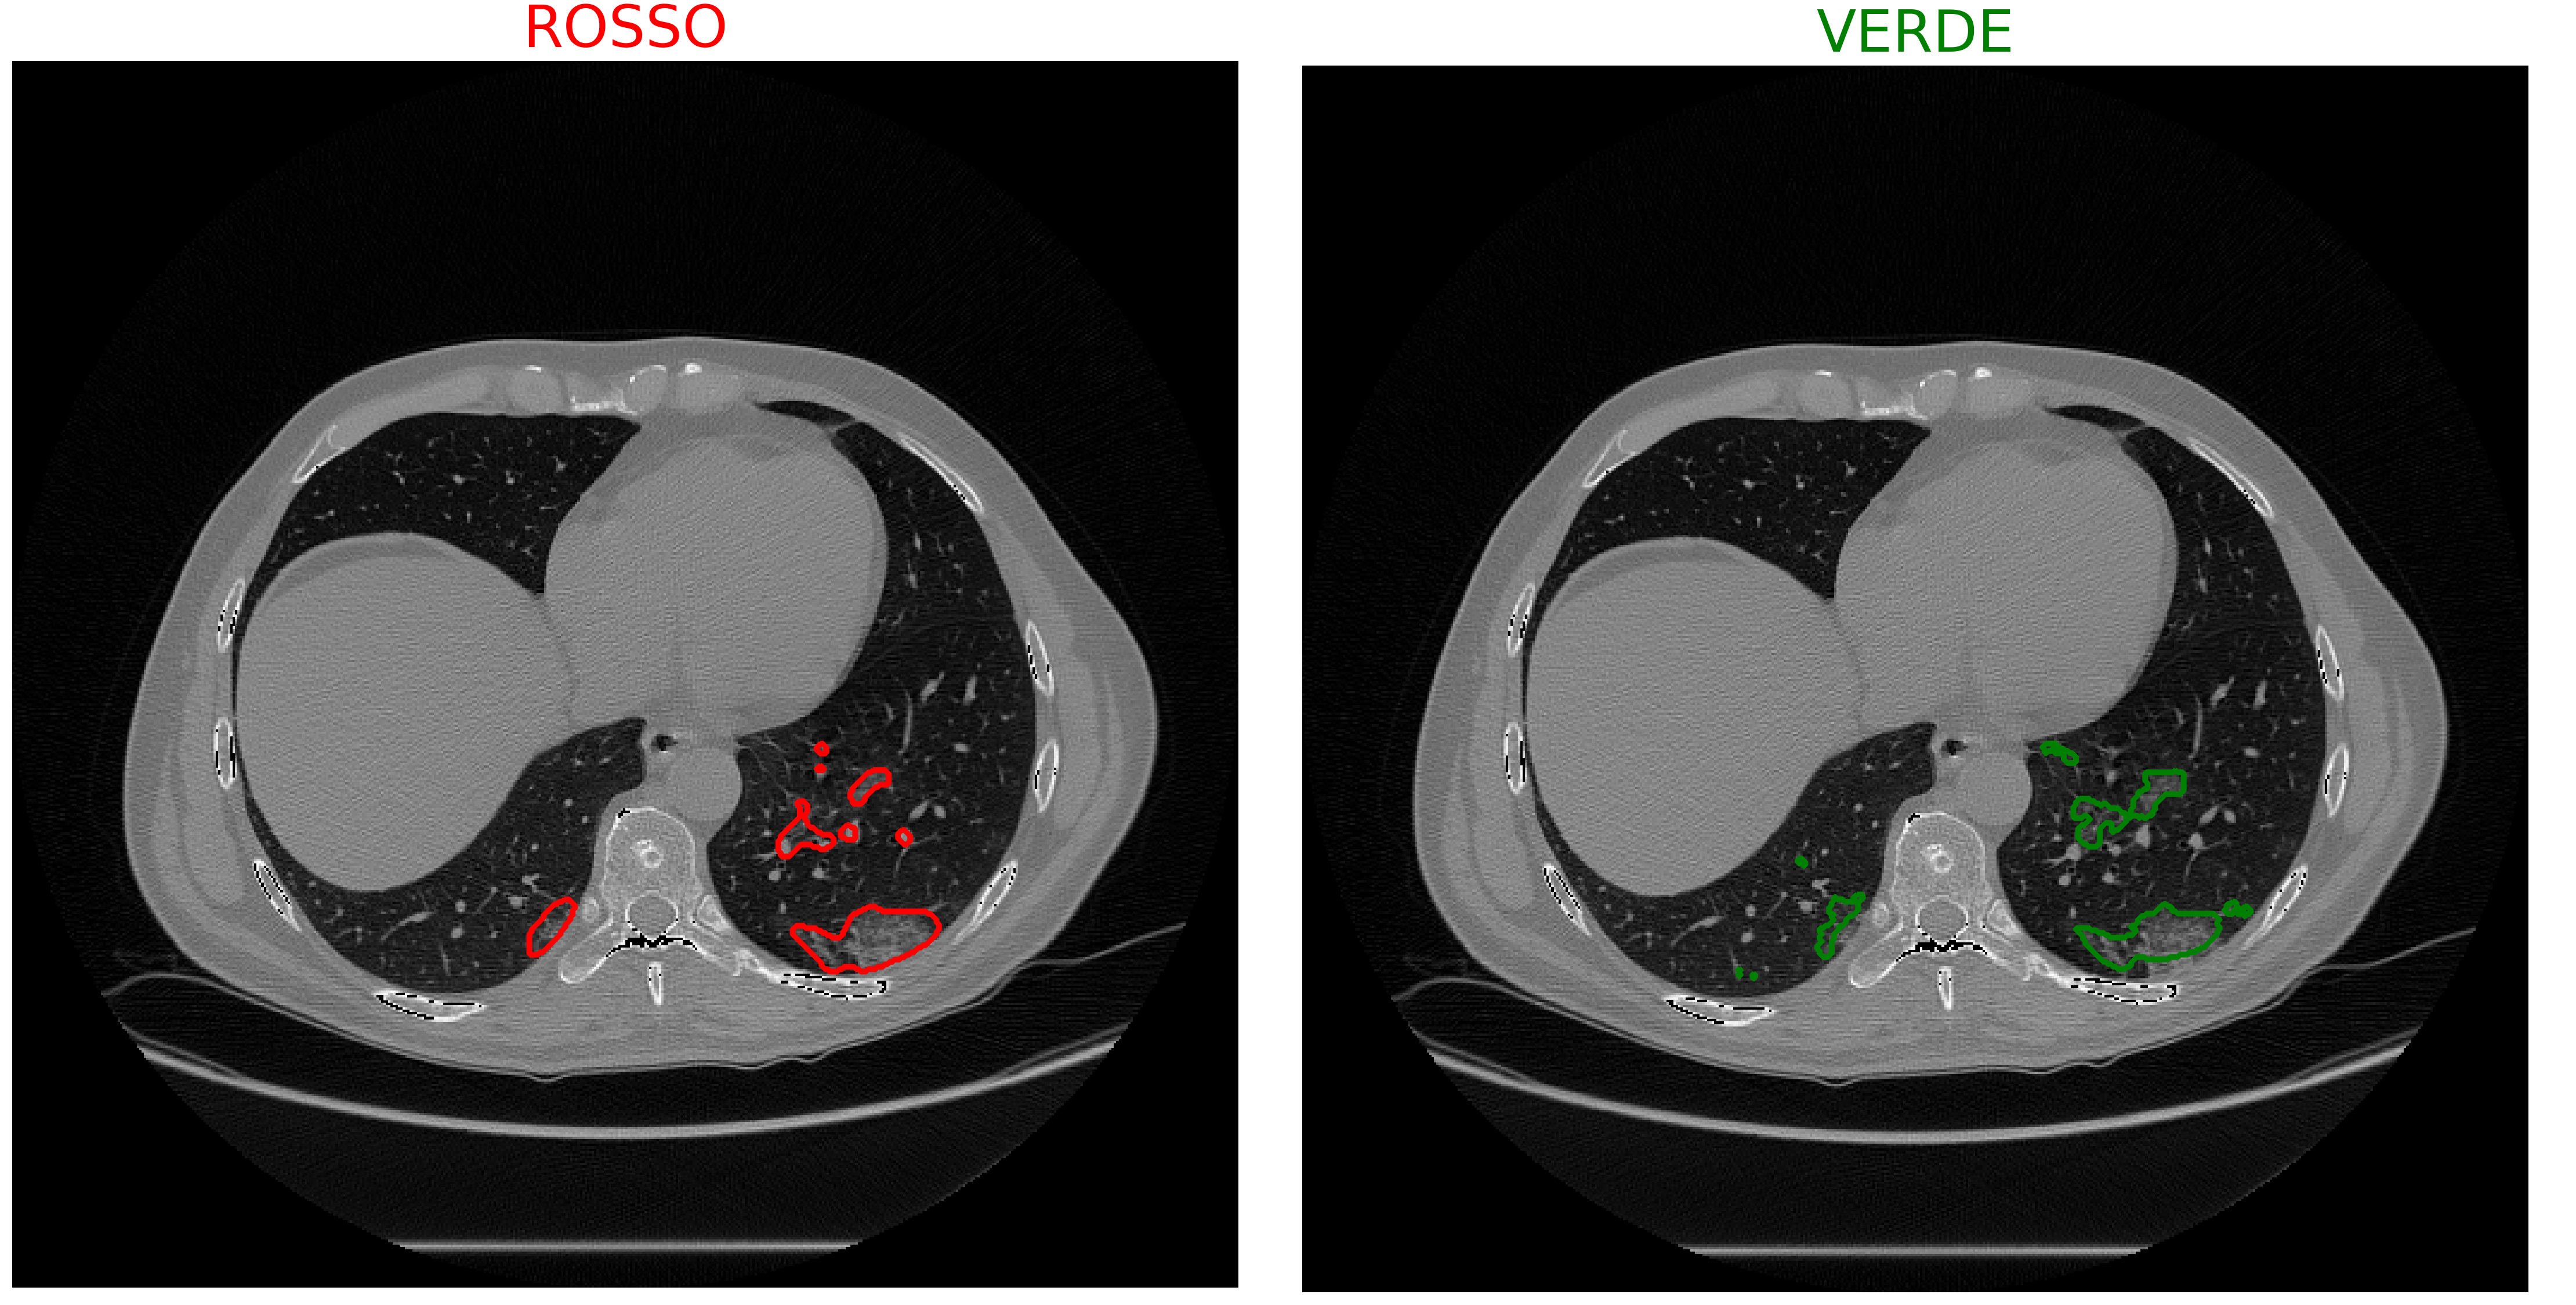
\includegraphics[scale=.3]{BlindEval.png}
			\caption{Example of comparison submitted to the experts. The two images report the segmentation of the same slices achieved with two different techniques: Manual and pipeline. Was asked to the expert to decide which one is better, without knowing which technique is used to obtain the segmentation.}\label{fig:Blind}
	\end{figure}

	The scans, organized in this way, was evaluated by experts, to which has been asked to decide for each which segmentation is better or if the quality is equal.
	
	The core of this method is that the expert don't know which scan corresponds to a specific segmentation technique, so this will lead to an ideally unbiased evaluation.  In order to ensure that, the order of segmentation was shuffled between patients. 
	
	

	
\end{document}